\documentclass{book}
\usepackage{lmodern}
\usepackage{amsmath}
\usepackage{amssymb}
\usepackage{amsfonts}
\usepackage{xcolor}
\usepackage{mdframed}
\usepackage[top=3cm, bottom=3cm, inner=4cm, outer=3cm]{geometry}
\usepackage{hhline}
\usepackage{graphicx}

\DeclareMathOperator{\lcm}{lcm}
\DeclareMathOperator{\bigo}{\mathcal{O}}
\renewcommand{\mod}{\textrm{mod }}

\newenvironment{task}
  {\begin{mdframed}[backgroundcolor=lightgray]}
  {\end{mdframed}}
  
\begin{document}

\chapter{Solutions}

\section{Multiples of 3 and 5}

\begin{task}
If we list all the natural numbers below $10$ that are multiples of $3$ and $5$, we get $3$, $5$, $6$, and $9$. The sum of these multiples is $23$.\\
\\
Find the sum of all the multiples of $3$ and $5$ below $1000$.
\end{task}

The first problem is pretty much straightforward. It asks us to find the sum of all multiples of $3$
and $5$, but any multiple must not exceed $1000 - 1 = 999$. But wait, is this task really that simple?
The only trick is that when we calculate the multiples, some of the multiples of $3$ and $5$ are the
same, e.g. $15$, $30$, ... That means, that if we do not implement this task in smart way, some of the
multiples might get counted twice. Those numbers are exactly the multiples of the least common
multiple of $3$ and $5$, which is $15$. We denote that as $\lcm(3, 5) = 15$.\\

Let us take a look at naive solution:

\begin{verbatim}
#include<stdio.h>

int main()
{
    int sum = 0;
    for (int i = 1; i <= 333; i++)   // we iterate from 1 to (int)999/3 = 333
        sum += 3 * i;
    for (int i = 1; i <= 199; i++)   // we iterate from 1 to (int)999/5 = 199
        sum += 5 * i;
    for (int i = 1; i <= 66; i++)    // we iterate from 1 to (int)999/15 = 66
        sum -= 15 * i;               // we must subtract the twice counted numbers
    printf("%d\n", sum);

    return 0;
}
\end{verbatim}

Note that if you implement this program, it will print the value instantly, therefore you might pose the question, why is this a naive solution?
The reasons are two. Firstly, we use three for loops. That results in asymptotic complexity of $\bigo(m/x + m/y + m/ \lcm(x, y))$, where $x$ and $y$ are the numbers whose multipliers we want to sum and $m$ is the upper bound for all multiples. Now consider we are given extremely large numbers. Although the program runs in linear time, it will take more and more time to get through those three loops. We can clearly see, that we could get rid of three loops and make only one loop, as in next implementation. Wait until you see the real reason why this implementation is not as beautiful as it could be (not to mention it is tiresomly slow - oh, wait, linear is slow, can you do it faster, let’s say logarithmic? Hell no, CONSTANT!).

\begin{verbatim}
#include<stdio.h>

int main()
{
    int sum = 0;
    for (int i = 3; i < 1000; i++)
    {
        if (i % 3 == 0 || i % 5 == 0)
            sum += i;
    }
    printf("%d\n", sum);
    
    return 0;
}
\end{verbatim}

Note that this implementation does not require any subtraction of multiples of $15$, because we check every integer between $3$ and $999$ inclusively only once. We also expect this program to run slower then the three for one, because in this case we have to loop through $m - 2 = 998$ numbers and each time check whether that number is a multiple of $3$ or $5$, whereas in three for loop we only loop through $\lfloor(m - 1)/x\rfloor + \lfloor(m - 1)/y\rfloor + \lfloor(m - 1)/ \lcm(x, y)\rfloor = 333 + 199 + 66 = 598$ numbers and we do not need to do any checks.

The second reason, and here starts the real solution to the problem, is that what we are doing is actually computing a sum of three \textit{arithmetic series}. An arithmetic series is a sum of numbers that are computed using relation \[a_1;~~~a_i = a_1 + d(i-1),\] where $d$ denotes a difference or \textit{distance} between two numbers in series. In our case we have three arithmetic series, first given by \[a_1 = 3;~~a_i = 3 + 3(i-1) = 3i,\] the second by \[b_1 = 5;~~b_i = 5 + 5(i-1) = 5i\] and the third by \[c_1 = 15;~~c_i = 15 + 15(i-1) = 15i.\] We are actually subtracting the sum of $\{c_i\}_{i = 1}^{66}$ series.
Now, beautiful mathematics gives us a formula for computing sum of arithmetic series. The formula is \[\sum_{i=1}^n a_i = \frac{n}{2}(a_1 + a_n).\] Since in our case $a_n = 3n$, $b_n = 5n$, and $c_n = 15n$, the above equation simplifies into \[\sum_{i=1}^n a_i = a_1 \cdot \frac{n(n+1)}{2}.\] You can simply make your own calculations to see that formula is indeed correct. Let us now implement the program WITHOUT any \texttt{for} loops at all! We use a formula derived above and get \[\textrm{sum} = \sum_{i=1}^{333} 3i + \sum_{i=1}^{199} 5i - \sum_{i=1}^{66} 15i = 3\cdot\frac{333\cdot334}{2} + 5\cdot\frac{199\cdot200}{2} - 15\cdot\frac{66\cdot67}{2}.\]

\begin{verbatim}
#include<stdio.h>
#include "campovski.h"               // needed for LCM

int main()
{
    int x, y, m;                     // we let user input starting numbers
    scanf("%d %d %d, &x, &y, &m);    // (in our case "3 5 1000")
    m--;                             // number below m, m not included (1000-1)
    
    int z = lcm(x, y);
    int n1 = (int) m / x;            // calculate range of sum for x (3)
    int n2 = (int) m / y;            // calculate range of sum for y (5)
    int n3 = (int) m / z;            // calculate range of sum for LCM(x,y) (15)
    
    int sum = x * n1 * (n1 + 1) / 2;
    sum += y * n2 * (n2 + 1) / 2;
    sum -= z * n3 * (n3 + 1) / 2;
    
    printf("%d\n", sum);
    
    return 0; 
}
\end{verbatim}

You might say taht you could do that faster with your own calculator. Well, the beauty of coding is finding mathematical background of given problem and optimizing the solution.\\

I tested all three of the above programs with number $x = 3$, $y = 5$, and $m \in \{10^3, 10^6, 10^9, 10^{12}\}$. The results are astounding (see table below). I also had to change \texttt{int}s to \texttt{long long}s.

\begin{table}[h!]
\centering
\begin{tabular}{||l||c|c|c|c||}
\hhline{|t:=====:t|}
\textit{Algorithm} & $t(m = 10^3)$ & $t(m = 10^6)$ & $t(m=10^9)$ & $t(m=10^{12})$\\
\hhline{||=||=|=|=|=||}
Three \texttt{for} loops & $0.000002$ & $0.001528$ & $1.384336$ & $1321.064965$\\
\hhline{||-||-|-|-|-||}
One \texttt{for} loop & $0.000004$ & $0.003579$ & $3.020462$ & \\
\hhline{||-||-|-|-|-||}
Formula & $< 0.000001$ & $< 0.000001$ & $< 0.000001$ & $< 0.000001$\\
\hhline{|b:=====:b|}
\end{tabular}
\caption{Table shows running time (in seconds) of given algorithms in relation to $m$. Time was measured with help of \texttt{time.h}.}
\end{table}

Note, hot lovely are the running times of first two algorithms increasing with $m$. Thousand times greater problem, thousand times more time needed. The third algorithm obviously runs in constant time.

\pagebreak

%%%%%%%%%%%%%%%%%%%%%%%%%%%%%%%%%%%%%%%%%%%%%%%%%%%%%%%%%%%%%%%%%%%%%%%%%%%%%%%%%%%%%%%%%%%%%%%%%%%%%%
%%%%%%%%%%%%%%%%%%%%%%%%%%%%%%%%%%%%%%%%%%%%%%%%%%%%%%%%%%%%%%%%%%%%%%%%%%%%%%%%%%%%%%%%%%%%%%%%%%%%%%
%%%%%%%%%%%%%%%%%%%%%%%%%%%%%%%%%%%%%%%%%%%%%%%%%%%%%%%%%%%%%%%%%%%%%%%%%%%%%%%%%%%%%%%%%%%%%%%%%%%%%%
%%%%%%%%%%%%%%%%%%%%%%%%%%%%%%%%%%%%%%%%%%%%%%%%%%%%%%%%%%%%%%%%%%%%%%%%%%%%%%%%%%%%%%%%%%%%%%%%%%%%%%

\section{Even Fibonacci numbers}

\begin{task}
Each new term in the Fibonacci sequence is generated by adding the previous two terms. By starting with $1$ and $2$, the first $10$ terms will be: \[1,2,3,5,8,13,21,34,55,89,\dotsc\]

By considering the terms in the Fibonacci sequence whose values do not exceed four million, find the sum of the even-valued terms.
\end{task}

Let us start with example from the task. The first ten terms of Fibonacci sequence, as the task states it, are $1$, $2$, $3$, $5$, $8$, $13$, $21$, $34$, $55$, and $89$. Even-valued terms, that do not exceed $34$ are $2$, $8$, and $34$. Therefore, the sum of the even-valued terms that do not exceed $34$ is $2+8+34 = 44$.\\

Before we get into programming, let us first discuss how terms of Fibonacci sequence are calculated. The first two terms, according to task, are $F_1 = 1$ and $F_2 = 2$. (Mind, that some sources state Fibonacci sequence as $1$, $1$, $2$, $3$, $5$, $8$, $13$,... or even $0$, $1$, $1$, $2$, $3$, $5$, $8$, $13$,...) The next term is acquired by adding previous two together. We end up with formula \[F_n = F_{n-1} + F_{n-2};~n \geq 3.\] This is recursive formula with starting values of $F_1 = 1$ and $F_2 = 2$. At this point you might think that we are going to recursion in order to calculate terms of Fibonacci sequence, but we are not. The reason is, that if we want to compute $n$-th term of Fibonacci sequence, we can use recursion. In our case, we do not know what term is the first that exceeds $4000000$, therefore we cannot use recursion. Besides, naive recursion (if we could use it) would calculate the same terms over and over again - see figure below. We could use a concept called \textit{memoization} and get rid of this problem, but as I said, we cannot use this technique in this situation.

\begin{figure}[h!]
\centering
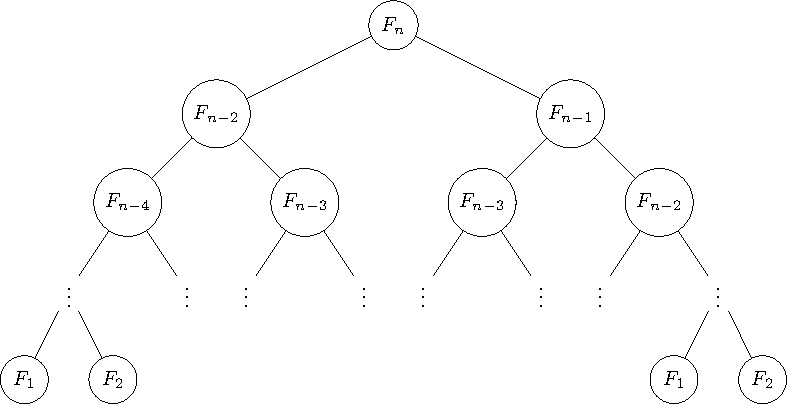
\includegraphics[scale=1]{images/002-tree.pdf}
\caption{Recursion tree for Fibonacci sequence. Note, how terms keep repeating.}
\end{figure}

Since we cannot use recursion from $n$ to $1$, we are going to go from $1$ to $n$, summing the previous two terms together to obtain the next one. We are going to check whether that term is even and if it is, we are going to add it to sum.

\begin{verbatim}
#include<stdio.h>

int main()
{
    int x = 1;             // x represents F(n-2)
    int y = 2;             // y represents F(n-1)
    int tmp;               // tmp represents F(n)
    int sum = 0;
    while (x <= 4000000)
    {
        if (!(x % 2))      // check if x is even
            sum += x;
        tmp = x + y;       // F(n) = F(n-1) + F(n-2)
        x = y;             // F(n-1) becomes F(n-2) for next iteration
        y = tmp;           // F(n) becomes F(n-1) for next iteration
    }
    printf("%d\n", sum);
    
    return 0;
}
\end{verbatim}

There are probably few things I should explain. First is the condition in \texttt{if} clause. In C, as well as in some other languages, number $0$ of type \texttt{int}, beside of being a regular number, stands for $\textit{false}$ (mind, that C does NOT have boolean variables). Thus, we do not need to make comparison of \texttt{0 == 0}, but we can simply write \texttt{!0}, which evaluates to \texttt{1}.
Next thing is the way we compute terms for next iteration. First, we sum current terms and save the result in temporary variable \texttt{tmp}. Then we rewrite \texttt{x} and \texttt{y} with \texttt{y} and \texttt{tmp} respectively, thus shifting the sequence to the left. The asymptotic complexity of this algorithm is $\bigo(n)$, where $n$ is the number which terms must not exceed - in our case $n = 4000000$.\\

Remember, that I said that some sources state Fibonacci sequence as $1$, $1$, $2$, $3$, $5$, $8$, $13$, $21$, $44$,... Observing this sequence for long enough we can see, that even-valued terms are $F_{3i}$ for all $i \in \mathbb{N}$. Proving this is simple. The sum of two odd numbers is even and the sum of even and odd number is odd. Looking at the sequence we can see that this proves the statement by law of induction. Therefore, we can be sure that if we add every third term of Fibonacci sequence to our final sum, we will obtain the correct result. The following algorithm does exactly that. Each iteration we compute the next three terms of Fibonacci sequence and always add the third to final sum.

\begin{verbatim}
#include<stdio.h>

int main()
{
    int x = 1;             // x represents F(n-2) - always odd
    int y = 1;             // y represents F(n-1) - always odd
    int z = 2;             // z represents F(n) - the even term
    int sum = 0;
    
    while (z <= 4000000)
    {
        sum += z;          // always add z since it is always even
        x = y + z;         // F(n+1) = F(n-1) + F(n) (x becomes F(n-2))
        y = z + x;         // F(n+2) = F(n) + F(n+1) (y becomes F(n-1))
        z = x + y;         // F(n+3) = F(n+2) + F(n+2) (z becomes F(n))
    }
    
    printf("%d\n", sum);
    
    return 0;
}
\end{verbatim}

This algorithm still runs in $\bigo(n)$ but we are advancing three times faster than in previous algorithm, because we calculate three terms in each iteration of \texttt{while} loop and omitting the \texttt{if} clause, thus expecting this algorithm to run approximately three times faster does not sound stupid. The only problem is that we are also doing more summations, which will result in algorithm not being three times as fast as the previous one, but it should still be faster.\\

Now it is time for some maths. We already figured out that even-valued terms are $F_{3i}$. If we manage to rewrite the recusrion formula $F_n = F_{n-1} + F_{n-2}$ into $F_n = \alpha f_{n-3} + \beta F_{n-6}$, we will obtain a formula that uses only every third Fibonacci number and we will not have to bother with odd-valued terms. Let us try to do that.
\begin{align*}
F_n &= F_{n-1} + F_{n-2}\\
&= (F_{n-2} + F_{n-3}) + (F_{n-3} + F_{n-4})\\
&= \big((F_{n-3} + F_{n-4}) + F_{n-3}\big) + \big(F_{n-3} + (F_{n-5} + F_{n-6})\big)\\
&= 3F_{n-3} + (F_{n-4} + F_{n-5}) + F_{n-6}\\
&= 4F_{n-3} + F_{n-6}
\end{align*}
Easy peasy lemon squizy! Based on formula derived, we can implement next program.

\begin{verbatim}
#include<stdio.h>

int main()
{
    int x = 2;             // x represents F(n-6)
    int y = 8;             // y represents F(n-3)
    int tmp;               // tmp represents F(n)
    int sum = 0;
    
    while (x <= 4000000)
    {
        sum += x;
        tmp = 4 * y + x;   // F(n) = 4 * F(n-3) + F(n-6)
        x = y;             // F(n-3) becomes F(n-6) for next iteration
        y = tmp;           // F(n) becomes F(n-3) for next iteration
    }
    
    printf("%d\n", sum);
    
    return 0;
}
\end{verbatim}

Can you guess, how much faster, if faster, will this algorithm run compared to the second one? It still runs in $\bigo(n)$, we still advance by three terms each iteration... But hey, did you forget about the number of operations again?! I hope not. This time, we do one multiplication more than in second algorithm, but two summations less. Therefore, we expect this program to run faster than the second one, and therefore also faster than the first one. Actually, if we compare the first program to the last one, we can see, that the difference is one \texttt{if} clause more in the first one and one small multiplication more in the third one. We might actually hope that the last algorithm will run three times as fast as the first one.\\

I ran all three programs and measured the time with \texttt{time.h} but the precision of timing was too low to see much difference. The first program finished in average time of $0.000002$ seconds, and the other two finished in under $0.000001$ seconds. with $n = 9\,000\,000\,000\,000\,000\,000 \approx \texttt{LLONG\_MAX}$ ($9$ quintillion). I decided to make each algorithm run more times. The following table shows the results.

\begin{table}[h!]
\centering
\begin{tabular}{||l||c|c|c||}
\hhline{|t:====:t|}
\textit{Algorithm} & $t(r = 10^3)$ & $t(r = 10^6)$ & $t(r = 10^9)$\\ \hhline{||=||=|=|=||}
\texttt{for} and \texttt{if} & $0.001498$ & $0.335005$ & $330.163120$\\ \hhline{||-||-|-|-||}
Naive three step & $0.000784$ & $0.183093$ & $181.040890$\\ \hhline{||-||-|-|-||}
Three step formula & $0.000215$ & $0.102709$ & $97.865098$\\ \hhline{|b:====:b|}
\end{tabular}
\caption{Table shows the running time (in seconds) of given algorithms in relation to $r$, where $r$ is the number of repetitions the core of program (the algorithm) ran. Time was measured with help of \texttt{time.h}.}
\end{table}

The results are just like we expected them to be. The \textit{three step formula} (last algorithm) is three times as fast as the \textit{\texttt{for} and \texttt{if}} (first algorithm). The \textit{naive three step} (second algorithm) is somewhere in the middle.

%%%%%%%%%%%%%%%%%%%%%%%%%%%%%%%%%%%%%%%%%%%%%%%%%%%%%%%%%%%%%%%%%%%%%%%%%%%%%%%%%%%%%%%%%%%%%%%%%%%%%%

\section{Largest prime factor}

\begin{task}
The prime factors of $13195$ are $5$, $7$, $13$, and $29$.\\
\\
What is the largest prime factor of the number $600851475143$?
\end{task}

There is a pretty straightforward solution to this problem that seemingly runs in $\bigo(n)$. What we can do is to loop through every number below $600851475143$ and check whether it is a prime and whether it divides $600851475143$. The most easily grasped solution with high running time. But why did I say it \textit{seemingly} runs in $\bigo(n)$. The answer is simple. We have to loop through $n$ numbers, for each check, whether it is a prime or not, that adds another $n$ in game. The total running time is then $\bigo(n^2)$. With $n = 600851475143$, my head starts burning. I just hope my computer will not. Let us implement this monstrous piece. I advise you not to try this at home. (Not sure should I do a backup first or not...)

\begin{verbatim}
#include<stdio.h>
#include<stdlib.h>
#define N 600851475143

int is_prime(long n);

int main()
{
    long largest = 1;
    for (long i = 2; i <= N; i++)
    {
        if (N % i == 0 && is_prime(i))
            largest = i;
    }

    printf("%li\n", largest);

    return 0;
}

int is_prime(long n)
{
    for (int i = 2; i < n; i++)
    {
        if (n % i == 0)
            return 0;
    }
    return 1;
}
\end{verbatim}

Mind two things: Although this is a not do at home algorithm, this might come in handy sometime in the future. Mind how we wrote \texttt{N \% i == 0} before \texttt{is\_prime(i)} in \texttt{if} clause of function \texttt{main}. Since we wrote it this way, the computer will first check whether \texttt{i} divides \texttt{N}. If not, it will not bother executing \texttt{is\_prime(i)}, since the \texttt{AND} clause will evaluate to \texttt{0} no matter the second argument. By doing that, we make sure, that we do not check every number for primality and therefore the running time of algorithm is reduced substantially. What we could also do is return $n$ when the for loop comes to it and \texttt{largest == 1}, since we did not find any other divisor of $n$, meaning $n$ is prime and we do not need to check its primality.

The second thing you should mind is that we do not need to check whether the new prime divisor is greater than the largest. You might have seen it by yourself why is so, but if not, here is the deal. The \texttt{i}, which is a possible prime divisor, increases and never decreases. Therefore, it always holds \texttt{i > largest}.\\

There are few things we could do better in implementation above and we would not even need to think hard. The first that comes to my mind is, that when we check for primality, we do not need to loop from $2$ to $n$. We only need to loop to $\sqrt{n}$. The reason is that if a number has a higher divisor then its square root, the result of division is smaller than number's square root and it is also a divisor. Therefore we can only check in range from $2$ to $\sqrt{n}$.\\

It is time for some maths. You have learned about \textit{sieve of Eratosthenes} in primary school for sure. The idea behind the sieve is to generate an array of numbers between $2$ and $n$. Then we start and cross out all multiples of $2$, except $2$, which is prime. After that, we cross out all multiples of next number that is not crossed, that is $3$. We continue by crossing the multiples of all numbers that are not crossed. By doing so, we end up with table of prime numbers. The array \texttt{eratosthenes} returns is the array of $0$s and $1$s. A $0$ on $i$-th place in array denotes $i$ is prime. For full implementation of Eratosthenes' sieve see appendix. The only problem is, that we cannot use it here, because we cannot store $600851475143$ bytes anywhere. We will have to dig further, but here is the implementation using sieve of Eratosthenes. It works for small numbers and it works fast.

\begin{verbatim}
#include<stdio.h>
#include "campovski.h"                  // needed for ERATOSTHENES
#define N 100003                        // some small number

int main()
{
    char* sieve = eratosthenes(N);      // get prime array
    int largest = 1;

    for (int i = 2; i <= N; i++)
    {
        if (!sieve[i] && N % i == 0)    // if i is prime, sieve[i] = 0
            largest = i;
    }

    printf("%d\n", largest);

    return 0;
}

\end{verbatim}

The idea for next algorithm comes directly from Eratosthenes but instead of creating a sieve, we completely divide out each of the divisor of $n$. By doing that we make sure that the next divisor will certainly be prime and therefore we do not need to check for divisor whether it is prime or not. By doing so we spare a lot of time, because every time we find a divisor $a$, we divide $n$ by $a$ as many times as we can, meaning we end up with smaller and smaller $n$, thus the calculation become faster and faster. Next implementation shows how that is done.

\begin{verbatim}
#include<stdio.h>
#include<stdlib.h>

int main()
{
    long long n = 600851475143;
    long long factor = 2;
    long long largest;

    while (n > 1)
    {
        if (!(n % factor))
        {
            largest = factor;
            do {
                n /= factor;
            } while (!(n % factor));
        }

        factor++;
    }

    printf("%lli\n", largest);

    return 0;
}
\end{verbatim}

This algorithm can be improved in two ways. It is obvious that $2$ is the only even-valued prime number. Therefore we can treat it on its own. By doing so, we can increase \texttt{factor} by 2 on each iteration and only traverse over odd numbers. The second improvement comes with realisation that every number can have at most one prime factor greater than $\sqrt{n}$. That leaves us with two options, either we found a factor lower then $\sqrt{n}$, divided it out and continued with next iteration, or we came to $\sqrt{n}$ and did not find a factor. In second option, we can stop checking since if there is no prime smaller then $n$ that would divide $n$, then the only numbers that divide $n$ are $1$ and $n$. That means $n$ is a prime and we return it. The next implementation does exactly that.

\begin{verbatim}
#include<stdio.h>
#include<math.h>

int main()
{
    long long n = 600851475143;
    long long largest = 1;

    if (!(n % 2))
    {
        largest = 2;
        do {
            n /= 2;
        } while (!(n % 2));
    }

    long long factor = 3;
    long long max_factor = (long long) sqrt(n);

    while (n > 1 && factor <= max_factor)
    {
        if (!(n % factor))
        {
            largest = factor;
            do {
                n /= factor;
            } while (!(n % factor));
            max_factor = (long long) sqrt(n);
        }

        factor += 2;
    }

    if (n == 1)
        printf("%lli\n", largest);
    else printf("%lli\n", n);

    return 0;
}
\end{verbatim}

I measured the running time of algorithms and the results were quite shocking. The first algorithm needed..., while the second and third one were surprisingly fast. The next table shows running times of algorithms with respect to $n$. Each program was run 1000 times to ensure smaller relative error, except for \textit{one step \texttt{factor}} on $n = 100123456789$.

\begin{table}[h!]
\centering
\begin{tabular}{||l||c|c|c|c|c||}
\hhline{|t:======:t|}
\textit{Algorithm} & $t(n = 10^3)$ & $t(n = 10^6)$ & $t(n = 10^5 + 3)$ & $t(n = n_1)$ & $t(n= n_2)$\\ \hhline{||=||=|=|=|=|=||}
Monster & $0.012390$ & $8.448938$ & $1.754996$ &  &\\ \hhline{||-||-|-|-|-|-||}
Sieve & $0.009984$ & $3.659880$ & $0.454618$ & $-$ & $-$ \\ \hhline{||-||-|-|-|-|-||}
One step \texttt{factor} & $0.000478$ & $0.000634$ & $0.214148$ & $0.130969$ & $\sim116$ days\\ \hhline{||-||-|-|-|-|-||}
Two step + \texttt{sqrt} & $0.006801$ & $0.007498$ & $0.001555$ & $0.023457$ & $1.362939$ \\ \hhline{|b:======:b|}
\end{tabular}
\caption{Table shows the running time (in seconds) of given algorithms with respect to $n$, where $n$ is the number whose greatest prime factor we are trying to calculate. $n_1 = 600851475143$ and $n_2 = 100123456789$ ($n_2$ is prime). Time was measured with help of \texttt{time.h}.}
\end{table}

As you can see, running times are quite strange. For small numbers that are not prime the \texttt{one step \texttt{factor}} is faster than \texttt{two step + \texttt{sqrt}}, because square root takes too much time to evaluate. On the other hand, if $n$ happens to be prime, the \texttt{one step \texttt{factor}} takes a lot of time, because it has to search through all numbers below $n$ before realizing it could actually return an answer. Therefore, one can clearly see that \textit{two step + \texttt{sqrt}} is a way to go. The \textit{sieve} is quite fast, but not appropriate for this problem, since has such a specific implementation that it simply cannot compete. We included it just for broadening mind. Mind also, that we computed sieve only once and ran the rest of the program 1000 times. Places with $-$ denote we could not allocate such a huge sieve and empty space means we did not run the program because it would take too long to execute.


%%%%%%%%%%%%%%%%%%%%%%%%%%%%%%%%%%%%%%%%%%%%%%%%%%%%%%%%%%%%%%%%%%%%%%%%%%%%%%%%%%%%%%%%%%%%%%%%%%%%%

\section{Largest palindrome product}

\begin{task}
A palindromic number reads the same both ways. The largest palindrome made from the product of two 2-digit numbers is $9009 = 91 \cdot 99$.\\
\\
Find the largest palindrome made from the product of two 3-digit numbers.
\end{task}

This task might look a bit awkward at first. The first problem we encounter is how to smartly generate possible products and the second is how to check if the number is palindrome.

We tackle the first problem in this way. For generating products we use two \texttt{for} loops to generate each number in product and then multiply them together. Since we are not stupid, we know that the product $x \cdot y$ is the same as $y \cdot x$. That means, that not both numbers $x$ and $y$ must start their loop at $100$. Instead, the inner loop can start where $x$ has left.

The second problem is a bit trickier. If we were to check if string is palindrome, we could simply iterate over it and check whether the $i$-th character from start is the same as $i$-th character from the end. In case of numbers, we cannot directly iterate over them, but have to first convert them into \texttt{char} arrays. We use function \texttt{int\_to\_arr}, which is defined in \texttt{campovski.h}. Now we can do what we would have done with strings. The other way is to use an algorithm for reversing the number and then checking if original number is the same as reversed, but we are not going to do that. Some other time maybe. If you are eager to learn, you can google how to reverse a number in C and you will get plenty of hits.\\

Now we are good to go implement the program.

\begin{verbatim}
#include<stdio.h>
#include<math.h>
#include<stdlib.h>
#include "campovski.h"          // needed for INT_TO_ARR

char is_palindrome(int n);

int main()
{
    int largest = 10000;        // 10000 = 100 * 100

    for (int x = 100; x <= 999; x++)
    {
        for (int y = x; y <= 999; y++)  // evade double checking
        {
            if (is_palindrome(x*y) && x * y >= largest)
                largest = x * y;
        }
    }

    printf("%d\n", largest);

    return 0;
}

char is_palindrome(int n)
{
    char* n_arr = int_to_arr(n);
    int l = floor(log10(abs(n))) + 1;
    for (int i = 0; i < (int) l/2; i++)
    {
        if (n_arr[i] != n_arr[l-i-1])
            return 0;
    }

    return 1;
}
\end{verbatim}

Although this program seems alright, there are still some improvements to make. First, let us assume that the largest palindrome product will be a product of two large 3-digit numbers. Therefore, we can start with $x = 999$, decrement $x$ on each iteration and break the inner \texttt{for} loop when $y$ is so small that $x * y \leq \textrm{largest}$. By doing that we hope to spend less time for finding the largest palindrome product.

The next improvemt is not always possible, therefore we will still consider the above program as BEST! This improvement comes after doing some maths. We realize that $111111 = 143\cdot 777$ is palindromic and $999 \cdot 999 < 1000000$. That means that the largest palindrome that is a product of two 3-digit numbers has 6 digits. Let $p$ be a palindromic number with 6 digits. Then we can write
\begin{align*}
p &= 100000a + 10000b + 1000c + 100c + 10b+ a\\
&= 100001a + 10010b + 1100c\\
&= 11(9091a + 910b + 100c)
\end{align*}

We figured out, that $11$ must divide the 6-digit palindrome. Since $11$ is a prime, a theorem from number theory and abstract algebra tells us, that at least one of $x$ and $y$ must be divisible by $11$. Therefore, if $x$ is not divisible by $11$, $y$ has to be. Using the information derived and described above, we can implement next program.

\begin{verbatim}
#include<stdio.h>
#include<stdlib.h>
#include<math.h>
#include "campovski.h"         // needed for INT_TO_ARR

char is_palindrome(int n);

int main()
{
    int largest = 111111;       // 111111 = 143 * 777
    int y, dy;

    for (int x = 999; x >= 100; x--)
    {
        if (x % 11 == 0)       // 11 divides x, doesn't need to divide y
        {
            y = 999;           // we must check all y's
            dy = 1;            // and decrement by 1
        }
        else                   // 11 must divide y
        {
            y = 990;           // largest 3 digit number that y % 11 = 0
            dy = 11;           // decrement by 11
        }

        for (; y >= x; y -= dy)
        {
            if (x * y <= largest)    // don't even need to check if
                break;               // the product is palindrome
            if (is_palindrome(x*y))
                largest = x * y;
           // y -= dy;
        }
    }

    printf("%d\n", largest);

    return 0;
}

char is_palindrome(int n)
{
    char* n_arr = int_to_arr(n);
    int l = floor(log10(abs(n))) + 1;
    for (int i = 0; i < (int) l/2; i++)
    {
        if (n_arr[i] != n_arr[l-i-1])
            return 0;
    }

    return 1;
}
\end{verbatim}

I tested the program above for finding the largest palindrome product of two $n$-digit numbers, where $n \in \{3,4,5\}$. The table above shows running times.

\begin{table}[h!]
\centering
\begin{tabular}{||l||c|c||}	
\hhline{|t:===:t|}
\textit{Algorithm} & $t(n=3)$ & $t(n=4)$\\ \hhline{||=||=|=||}
Simple & $0.140$ & $5.852$ \\ \hhline{||-||-|-||}
Advanced & $0.086 / 1000$ & \\ \hhline{|b:===:b|}
\end{tabular}
\caption{Running time (in seconds) of two implementations for finding largest palindromic product of two $n$-digit numbers. The time was measured by \texttt{time} command in bash shell.}
\end{table}

As we assumed the second algorithm was much faster, but it could not be used in case of $n = 4$, since the product of two 4-digit numbers can either be a 7-digit or 8-digit number. We could of course break that down too and maybe find something interesting but we are not going to. You can do that for your homework.\\

From now on, we will be measuring running time with Unix \texttt{time} command rather than with \texttt{time.h}.


%%%%%%%%%%%%%%%%%%%%%%%%%%%%%%%%%%%%%%%%%%%%%%%%%%%%%%%%%%%%%%%%%%%%%%%%%%%%%%%%%%%%%%%%%%%%%%%%%%%%%

\section{Smallest multiple}

\begin{task}
$2520$ is the smallest number that can be divided by each of the numbers from $1$ to $10$ without any remainder.\\
\\
What is the smallest positive number that is evenly divisible by all of the numbers from $1$ to $20$?
\end{task}

This is the first task that actually requires us to know some maths. There is no naive implementation that would just pop up from nowhere. What this task actually requires is to solve the next system of linear congruences:
\begin{align*}
n &\equiv 0~(\mod 1)\\
n &\equiv 0~(\mod 2)\\
n &\equiv 0~(\mod 3)\\
&~~\vdots\\
n &\equiv 0~(\mod 20)
\end{align*}

The only thing we are lucky here is, that $n$ has to be congruent to $0$ by all moduli. The reason for that is, that if $x$ was to be congruent to some other numbers, we would have to use \textit{Chinese remainder theorem}. And since Chinese remainder theorem only works when moduli are pairwise coprime, meaning that $\gcd$ of each pair of moduli is $1$, we would have to disassemble the pairs of congruences where $\gcd$ of moduli would not be $1$ into more congruences whose moduli would be pairwise coprime. The reason why we do not need to use Chinese remainder theorem is fairly obvious. Since $n$ has to be congruent to $0$, that means that $n$ has to be a multiple of moduli. Because we are looking for the smallest number that satisfies these criteria, we are actually looking for least common multiple of moduli. Once we know that, the implementation is really easy, just like "Hello world!".\\

Let me just mention few things on how to implement the algorithm. First, since $1$ divides every number, we can omit the first congruence. Second, the following is true and can be easily proved: \[\lcm(x,y,z) = \lcm(\lcm(x,y), z) = \lcm(x, \lcm(y,z)).\] We can use that to compute $\lcm$ on-the-fly, meaning we can compute the $\lcm$ of previous $\lcm$ and next modulo and the result will be the $\lcm$ of all moduli.

\begin{verbatim}
#include<stdio.h>
#include "campovski.h"                // used for LCM

int main()
{
    int r = 20;                       // the highest modulo is 20
    long long n = 2;                  // 1 divides everything

    for (int i = 3; i < r; i++)
        n = lcm(n, i);                // compute lcm of moduli

    printf("%lli\n", n);

    return 0;
}
\end{verbatim}

This algorithm is faster than light. I ran it with different $r$s and the following table shows the results.

\begin{table}[h!]
\centering
\begin{tabular}{||l||c|c|c||}
\hhline{|t:====:t|}
\textit{Algorithm} & $t(r = 20)$ & $t(r = 30)$ & $t(r = 40)$ \\ \hhline{||=||=|=|=||}
\texttt{lcm} & $0.676 \times 10^{-6}$ & $1.112 \times 10^{-6}$ & $1.508 \times 10^{-6}$ \\ \hhline{|b:====:b|}
\end{tabular}
\caption{Running time (in seconds) of the algorithm, measured by Unix \texttt{time} bash command.}
\end{table}

The limit on $r$ is $r = 43$. With $r >= 44$ we cannot store $n$ in \texttt{unsigned long long}. Note, that \textit{Project Euler Problem 5 overview} contains different algorithm, but that algorithm is highly impractical. The reason is, that the algorithm assumes it is given an array of prime numbers, which takes time to calculate. Furthermore, we cannot use our \texttt{eratosthenes} from \texttt{campovski.h} because that array contains a lot of zeros and uses a lot of important memory. We would need to implement another function that can compute large primes in a moment and return the array prime numbers. We might do that in the future, if we come across some high primality problem.

The algorithm provided by Project Euler is suitable for extremely large numbers, which you would need to store in \texttt{char} array but we are not going to go into that at this moment. If you want you can check the algorithm after you have succesfully solved the problem and checked the solution.

%%%%%%%%%%%%%%%%%%%%%%%%%%%%%%%%%%%%%%%%%%%%%%%%%%%%%%%%%%%%%%%%%%%%%%%%%%%%%%%%%%%%%%%%%%%%%%%%%%%%%

\section{Sum square difference}

\begin{task}
The sum of the squares of the first ten natural numbers is \[1^2 + 2^2 + \dotsm + 10^2 = 385.\] The square of the sum of the first ten natural numbers is \[(1+2+ \dotsm + 10) ^2 + 55^2 = 3025.\] Hence the difference between the sum of the squares of the first ten natural numbers and the square of the sum is $3025 - 385 = 2640$.\\
\\
Find the difference between the sum of the squares of the first one hundred natural numbers and the square of the sum.
\end{task}

This task is really simple. Even a child in primary school can solve it. All you have to do is loop from numbers between $1$ and $100$, calculate their squares and add that number to final sum At the same time we add each number to \texttt{tmp} which is a normal sum of integers between $1$ and $100$. At the end we subtract the normal sum squared from the sum of squares and print a number that is greater than $0$. BAM, problem 6 done!

\begin{verbatim}
#include<stdio.h>

int main()
{
    int sum = 0;                            // sum of squares
    int tmp = 0;                            // sum of natural
    for (int i = 1; i <= 100; i++)
    {
        sum += i * i;
        tmp += i;
    }
    sum -= tmp * tmp;                       // calculate difference

    printf("%d\n", sum >= 0 ? sum : -sum);  // print nonnegative sum

    return 0;
}
\end{verbatim}

But wait, there must be something behind this problem. It cannot be that easy and the straightforward solution shall not return the answer instantly... Actually there is a better solution. The implementation above runs in $\bigo(n)$. But since this is a simple mathematical problem, there exists a solution that runs in $\bigo(1)$. Let me walk you to better solution.\\

In \textit{problem 1} we already discussed the concept of \textit{arithmetic series}. The sum of natural numbers between $1$ and $n$ is nothing else but an arithmetic series with $a_1 = 1$ and $d = 1$. So we derive the next formula: \[\sum_{i=1}^n i = \frac{n(n+1)}{2}.\] For the sum of squares, there also exists a formula, which we are not going to derive here but the derivation can easily be found online. The formula is \[\sum_{i=1}^n i^2 = \frac{n(n+1)(2n+1)}{6}.\] Once known it can be quite easily proved by the law of induction. Knowing this two formulas, we get a solution that runs in $\bigo(1)$.

\begin{verbatim}
#include<stdio.h>

int main()
{
    int n = 100;
    int sum_squares = n * (n+1) * (2*n+1) / 6;  // sum of squares
    int sum = n * (n+1) / 2;                    // sum of natural
    int diff = sum_squares - sum * sum;         // difference

    printf("%d\n", diff >= 0 ? diff : -diff);   // print nonnegative diff

    return 0;
}
\end{verbatim}

Mind, that we did not need the extra variable \texttt{diff}. We only did that to make the code more readable. Another thing we could do in some other situation is, that we could divide by 6 in \texttt{sum\_squares} at some other position and by that evade the number from growing over the result of that whole line operation, thus being able to calculate higher sums since we would not overflow. But in this case we cannot do that, since we do not know whether any of numbers $n$, $n+1$, and $2n+1$ is divisible by $6$. I am just saying this so you know that the order of operation matters and can sometimes get really useful. For example, if we knew that $n$ is even, we could write \texttt{int sum = n / 2 * (n+1);} and may be able to calculate sum for higher $n$, because we would first halve the $n$ and then multiply it by $n+1$. Similarly, if $n$ was even, we could write \texttt{int sum = (n+1) / 2 * n;}.

I ran the above programs and measured running time with Unix \texttt{time}. The results are in the following table.

\begin{table}[h!]
\centering
\begin{tabular}{||l||c|c|c||}
\hhline{|t:====:t|}
\textit{Algorithm} & $t(n=10^2)$ & $t(n = 10^3)$ & $t(n=10^4)$\\ \hhline{||-||---||}
Brute force & $0.384 \times 10^{-6}$ & $2.964 \times 10^{-6}$ & $29.340 \times 10^{-6}$\\ \hhline{||-||---||}
Formulas & $0.016 \times 10^{-6}$ & $0.012 \times 10^{-6}$ & $0.024 \times 10^{-6}$ \\ \hhline{|b:====:b|}
\end{tabular}
\caption{Running time (in seconds) of programs. They were run $10^6$-times, that is why the time is then divided by $10^6$. $n$ is the upper range of the sum we are calculating (from $1$ to $n$).}
\end{table}

One can clearly see, that first program is nicely linear in $n$. The second runs in constant time... Actually it runs in some respect to the length of $n$, since the longer the number, the more time it needs to multiply. But that is still $\bigo(1)$ with respect to $n$.

%%%%%%%%%%%%%%%%%%%%%%%%%%%%%%%%%%%%%%%%%%%%%%%%%%%%%%%%%%%%%%%%%%%%%%%%%%%%%%%%%%%%%%%%%%%%%%%%%%%%%

\section{10001st prime}

\begin{task}
By listing the first six prime numbers: $2$, $3$, $5$, $7$, $11$, and $13$, we can see that the 6th prime is $13$.\\
\\
What is the 10001st prime number?
\end{task}

We have already discussed a great deal about prime numbers in \textit{problem 3}. Therefore, we are not going to go in any details here. We are going to use \texttt{eratosthenes} from \texttt{campovski.h} which starts with array of $0$ and then places $1$ on $i$-th place if $i$ is NOT a prime number.

After acquiring the eratosthenes sieve, we loop through it and every time we find $0$ we add $1$ to count of prime numbers. When count reaches $10001$, we stop and print the index. If the returned index is \texttt{i = len(sieve) - 1}, the sieve made is not big enough, because we now that \texttt{(len(sieve) - 1} is not a prime number, since it is even.

\begin{verbatim}
#include<stdio.h>
#include "campovski.h"

int main()
{
    char* sieve = eratosthenes(1000001);  // generate huge sieve
    int count = 0;                        // count of primes

    int i;                                // we will need i outside the loop
    for (i = 2; i < 1000001; i++)
    {
        if (!sieve[i])                    // if sieve[i] = 0 then i is prime
            count++;                      // we found another prime
        if (count == 10001)               // we found 10001st prime
            break;
    }

    printf("%d\n", i);

    return 0;
}
\end{verbatim}

Let us take a look at the running times of above implementation with different $n$s, where $n$ means that we want to find $n$-th prime.

\begin{table}[h!]
\centering
\begin{tabular}{||l||c|c|c|c||}
\hhline{|t:=====:t|}
\textit{Algorithm} & $t(n=10001)$ & $t(n = 10^5)$ & $t(n=10^6)$ & $t(n=10^7)$\\ \hhline{||-||----||}
Sieve walk & $0.048$ & $0.236$ & $2.700$ & $29.080$ \\ \hhline{|b:=====:b|}
\end{tabular}
\caption{Running time (in seconds) of programs. We used a sieve of size $10^6 + 1$ for $n=10001$, $10^7 + 1$ for $n = 10^5$, $10^8 + 1$ for $n = 10^6$. and $10^9 + 1$ for $n = 10^7$.}
\end{table}

The algorithm is lovely linear. We increase $n$ ten times, the running time increases ten times.


%%%%%%%%%%%%%%%%%%%%%%%%%%%%%%%%%%%%%%%%%%%%%%%%%%%%%%%%%%%%%%%%%%%%%%%%%%%%%%%%%%%%%%%%%%%%%%%%%%%%%
\setcounter{section}{24}
\section{1000-digit Fibonacci number}

\begin{task}
The Fibonacci sequence is defined by the recurrence relation:
\[F_n = F_{n-1} + F_{n-2},\textrm{ where $F_1 = 1$ and $F_2 = 1$}.\]
Hence the first $12$ terms will be:
\begin{align*}
F_1 &= 1\\
F_2 &= 1\\
F_3 &= 2\\
F_4 &= 3\\
F_5 &= 5\\
F_6 &= 6\\
F_7 &= 13\\
F_8 &= 21\\
F_9 &= 34\\
F_{10} &= 55\\
F_{11} &= 89\\
F_{12} &= 144
\end{align*}
The $12$th term, $F_{12}$, is the first term to contain three digits.\\
\\
What is the index of the first term in the Fibonacci sequence to contain $1000$ digits?
\end{task}

This is one of the problems that we are particularly not lucky to be programming in C. We cannot store the $1000$ digit number in any of number types. We will have to use array of \texttt{int}s (we could use \texttt{char}s, but it is really not necessary, since we do not need to spare with memory). The only possible solution to this problem is brute force, since there are no known rules for how Fibonacci numbers' lengths increase. In languages like Python we could write the solution to this problem very easily because we do not need to worry about storing such huge numbers. The solution in Python is this:

\begin{verbatim}
x = 1
y = 1
count = 2
while len(str(y)) != 1000:
    x, y = y, x + y
    count += 1
print count
\end{verbatim}

Simple as f***. Now, the solution in C is not much harder, we just have to be careful with arrays. Since we will not care about memory, we can allocate three $1000$ \texttt{int}s long arrays, one for $F_{n-1}$, one for $F_n$, and one for $F_{n+1}$. Then we loop over all the digits in $F_{n-1}$ and $F_n$ and calculate each digit of $F_{n+1}$ by piece. The only problem is, that we must take care of the situation where \texttt{F(n-1)[i] + F(n)[i] >= 10}. In this case, we have to remember to increment the next digit. Fairly simple, but quite painful. The next implementation does exactly that.

\begin{verbatim}
#include<stdio.h>
#include<stdlib.h>

int main()
{
    int* x = (int*) malloc(1000*sizeof(int));
    int* y = (int*) malloc(1000*sizeof(int));
    int* tmp = (int*) malloc(1000*sizeof(int));
    int inc = 0;                                  // increment on next step

    x[0] = 1;                                     // F(1) = 1
    y[0] = 1;                                     // F(2) = 1
    int count = 2;                                // we already know 2 numbers

    while (!y[999])                               // loop while 1000th digit is 0
    {
        for (int i = 0; i < 1000; i++)
        {
            int s = x[i] + y[i] + inc;            // sum of i-th digit + increment
            tmp[i] = s % 10;                      // digit of F(n+1)
            x[i] = y[i];                          // F(n) becomes F(n-1)
            y[i] = tmp[i];                        // F(n+1) becomes F(n)
            inc = (s >= 10) ? 1 : 0;              // if s>=10, we must inc on next iter
        }
        count++;
    }

    printf("%d\n", count);

    return 0;
}
\end{verbatim}

Now if we would want to spare with memory, we would have two options. The first thing we could do is change all \texttt{int} values to \texttt{short}s. That would spare a lot of the memory we used for variables. But furthermore, since we know that we will only be using really small numbers at a time (less then $9+9+1 = 19$), we could allocate a \texttt{char} array and spare even more. Many people think that \texttt{char} stands for \textit{character}. Well, it actually does, but the \texttt{char} type can normally store integral values, just as long as they do not exceed $2^8$. Instead of $4$ bytes (can store up to $2^{32}$) for an \texttt{int}, we could only use $1$ byte (can store up to $2^8$) for a \texttt{char}. The implementation is the same.

\begin{verbatim}
#include<stdio.h>
#include<stdlib.h>

int main()
{
    char* x = (char*) malloc(1000*sizeof(char));
    char* y = (char*) malloc(1000*sizeof(char));
    char* tmp = (char*) malloc(1000*sizeof(char));
    char inc = 0;

    x[0] = 1;
    y[0] = 1;
    int count = 2;

    while (!y[999])
    {
        for (int i = 0; i < 1000; i++)
        {
            char s = x[i] + y[i] + inc;
            tmp[i] = s % 10;
            x[i] = y[i];
            y[i] = tmp[i];
            inc = s >= 10 ? 1 : 0;
        }
        count++;
    }

    printf("%d\n", count);

    return 0;
}
\end{verbatim}

Let me take another note on \texttt{char}s. One \texttt{char} is 1 byte, 1 byte is 8 bits and 1 bit can store two values, \texttt{0} and \texttt{1}. Since we can store 8 bits in a byte, that means, we can store $2^8$ values in 1 byte. Therefore, if we only have less than $2^8 = 256$ different signs to store, we can use a \texttt{char}. We use so called ASCII table, which is nothing else but a bijection between symbols like characters, numbers, punctuation, etc. and numbers between $0$ and $255$. For example, a character \texttt{"A"} has an ASCII value of \texttt{65}. Therefore, if we write something like \texttt{char c = "A";}, what actually gets stored in \texttt{c} is the number \texttt{65}, which represents \texttt{"A"}. That means, that if we store \texttt{42} in \texttt{char}, the computer might understand that as a character with ASCII value of 42, that is \texttt{*}, but it can serve as a pure number for our needs, see what I mean? For full ASCII table go ahead and google it, there is really no point in creating one here.

Also, we will not be making any time comparison here, since we only have one algorithm, the running time of which is clearly $\bigo(n)$, where $n$ is the length of Fibonacci number, in our case $n = 1000$.\\

I measured the running times of above programs with Unix \texttt{time} bash command. The following table contains results.

\begin{table}[h!]
\centering
\begin{tabular}{||l||c|c|c||}
\hhline{|t:====:t|}
\textit{Algorithm} & $t(n=10^3)$ & $t(n=10^4)$ & $t(n=10^5)$\\ \hhline{||=||=|=|=||}
\texttt{int*} & $0.076$ & $4.004$ & $398.320$ \\ \hhline{||-||-|-|-||}
\texttt{char*} & $0.040$ & $4.064$ & $402.524$ \\ \hhline{|b:====:b|}
\end{tabular}
\caption{Running times of the implementations with respect to $n$, where $n$ is the desired length of Fibonacci number.} 
\end{table}




































\end{document}
